\documentclass[10pt,a4paper]{article}
\usepackage{blindtext}
\usepackage{subcaption}
\usepackage{graphicx}
\usepackage{tikz}
\usepackage{amssymb}
\usepackage{caption}
\usepackage{amsmath}
\usepackage{circuitikz}
\usepackage{hyperref}
\usepackage{amssymb}
\usepackage[spanish,activeacute,es-tabla]{babel}
\usepackage[utf8]{inputenc}
\usepackage{ifthen}
\usepackage{listings}
\usepackage{dsfont}
\usepackage{subcaption}
\usepackage{amsmath}
\usepackage[strict]{changepage}
\usepackage[top=1cm,bottom=2cm,left=1cm,right=1cm]{geometry}%
\usepackage{color}%
\newcommand{\tocarEspacios}{%
	\addtolength{\leftskip}{3em}%
	\setlength{\parindent}{0em}%
}

% Especificacion de procs

\newcommand{\In}{\textsf{in }}
\newcommand{\Out}{\textsf{out }}
\newcommand{\Inout}{\textsf{inout }}

\newcommand{\encabezadoDeProc}[4]{%
	% Ponemos la palabrita problema en tt
	%  \noindent%
	{\normalfont\bfseries\ttfamily proc}%
	% Ponemos el nombre del problema
	\ %
	{\normalfont\ttfamily #2}%
	\
	% Ponemos los parametros
	(#3)%
	\ifthenelse{\equal{#4}{}}{}{%
		% Por ultimo, va el tipo del resultado
		\ : #4}
}

\newenvironment{proc}[4][res]{%
	
	% El parametro 1 (opcional) es el nombre del resultado
	% El parametro 2 es el nombre del problema
	% El parametro 3 son los parametros
	% El parametro 4 es el tipo del resultado
	% Preambulo del ambiente problema
	% Tenemos que definir los comandos requiere, asegura, modifica y aux
	\newcommand{\requiere}[2][]{%
		{\normalfont\bfseries\ttfamily requiere}%
		\ifthenelse{\equal{##1}{}}{}{\ {\normalfont\ttfamily ##1} :}\ %
		\{\ensuremath{##2}\}%
		{\normalfont\bfseries\,\par}%
	}
	\newcommand{\asegura}[2][]{%
		{\normalfont\bfseries\ttfamily asegura}%
		\ifthenelse{\equal{##1}{}}{}{\ {\normalfont\ttfamily ##1} :}\
		\{\ensuremath{##2}\}%
		{\normalfont\bfseries\,\par}%
	}
	\renewcommand{\aux}[4]{%
		{\normalfont\bfseries\ttfamily aux\ }%
		{\normalfont\ttfamily ##1}%
		\ifthenelse{\equal{##2}{}}{}{\ (##2)}\ : ##3\, = \ensuremath{##4}%
		{\normalfont\bfseries\,;\par}%
	}
	\renewcommand{\pred}[3]{%
		{\normalfont\bfseries\ttfamily pred }%
		{\normalfont\ttfamily ##1}%
		\ifthenelse{\equal{##2}{}}{}{\ (##2) }%
		\{%
		\begin{adjustwidth}{+5em}{}
			\ensuremath{##3}
		\end{adjustwidth}
		\}%
		{\normalfont\bfseries\,\par}%
	}
	
	\newcommand{\res}{#1}
	\vspace{1ex}
	\noindent
	\encabezadoDeProc{#1}{#2}{#3}{#4}
	% Abrimos la llave
	\par%
	\tocarEspacios
}
{
	% Cerramos la llave
	\vspace{1ex}
}

\newcommand{\aux}[4]{%
	{\normalfont\bfseries\ttfamily\noindent aux\ }%
	{\normalfont\ttfamily #1}%
	\ifthenelse{\equal{#2}{}}{}{\ (#2)}\ : #3\, = \ensuremath{#4}%
	{\normalfont\bfseries\,;\par}%
}

\newcommand{\pred}[3]{%
	{\normalfont\bfseries\ttfamily\noindent pred }%
	{\normalfont\ttfamily #1}%
	\ifthenelse{\equal{#2}{}}{}{\ (#2) }%
	\{%
	\begin{adjustwidth}{+2em}{}
		\ensuremath{#3}
	\end{adjustwidth}
	\}%
	{\normalfont\bfseries\,\par}%
}

% Tipos

\newcommand{\nat}{\ensuremath{\mathds{N}}}
\newcommand{\ent}{\ensuremath{\mathds{Z}}}
\newcommand{\float}{\ensuremath{\mathds{R}}}
\newcommand{\bool}{\ensuremath{\mathsf{Bool}}}
\newcommand{\cha}{\ensuremath{\mathsf{Char}}}
\newcommand{\str}{\ensuremath{\mathsf{String}}}

% Logica

\newcommand{\True}{\ensuremath{\mathrm{true}}}
\newcommand{\False}{\ensuremath{\mathrm{false}}}
\newcommand{\Then}{\ensuremath{\rightarrow}}
\newcommand{\Iff}{\ensuremath{\leftrightarrow}}
\newcommand{\implica}{\ensuremath{\longrightarrow}}
\newcommand{\IfThenElse}[3]{\ensuremath{\mathsf{if}\ #1\ \mathsf{then}\ #2\ \mathsf{else}\ #3\ \mathsf{fi}}}
\newcommand{\yLuego}{\land _L}
\newcommand{\oLuego}{\lor _L}
\newcommand{\implicaLuego}{\implica _L}

\newcommand{\cuantificador}[5]{%
	\ensuremath{(#2 #3: #4)\ (%
		\ifthenelse{\equal{#1}{unalinea}}{
			#5
		}{
			$ % exiting math mode
			\begin{adjustwidth}{+2em}{}
				$#5$%
			\end{adjustwidth}%
			$ % entering math mode
		}
		)}
}

\newcommand{\existe}[4][]{%
	\cuantificador{#1}{\exists}{#2}{#3}{#4}
}
\newcommand{\paraTodo}[4][]{%
	\cuantificador{#1}{\forall}{#2}{#3}{#4}
}

%listas

\newcommand{\TLista}[1]{\ensuremath{seq \langle #1\rangle}}
\newcommand{\lvacia}{\ensuremath{[\ ]}}
\newcommand{\lv}{\ensuremath{[\ ]}}
\newcommand{\longitud}[1]{\ensuremath{|#1|}}
\newcommand{\cons}[1]{\ensuremath{\mathsf{addFirst}}(#1)}
\newcommand{\indice}[1]{\ensuremath{\mathsf{indice}}(#1)}
\newcommand{\conc}[1]{\ensuremath{\mathsf{concat}}(#1)}
\newcommand{\cab}[1]{\ensuremath{\mathsf{head}}(#1)}
\newcommand{\cola}[1]{\ensuremath{\mathsf{tail}}(#1)}
\newcommand{\sub}[1]{\ensuremath{\mathsf{subseq}}(#1)}
\newcommand{\en}[1]{\ensuremath{\mathsf{en}}(#1)}
\newcommand{\cuenta}[2]{\mathsf{cuenta}\ensuremath{(#1, #2)}}
\newcommand{\suma}[1]{\mathsf{suma}(#1)}
\newcommand{\twodots}{\ensuremath{\mathrm{..}}}
\newcommand{\masmas}{\ensuremath{++}}
\newcommand{\matriz}[1]{\TLista{\TLista{#1}}}
\newcommand{\seqchar}{\TLista{\cha}}

\renewcommand{\lstlistingname}{Código}
\lstset{% general command to set parameter(s)
	language=Java,
	morekeywords={endif, endwhile, skip},
	basewidth={0.47em,0.40em},
	columns=fixed, fontadjust, resetmargins, xrightmargin=5pt, xleftmargin=15pt,
	flexiblecolumns=false, tabsize=4, breaklines, breakatwhitespace=false, extendedchars=true,
	numbers=left, numberstyle=\tiny, stepnumber=1, numbersep=9pt,
	frame=l, framesep=3pt,
	captionpos=b,
}


\title{Sistemas Digitales}
\author{Tomás Agustín Hernández}
\date{}

\begin{document}
\maketitle


\begin{figure}[b]
    \centering
    \begin{tikzpicture}[remember picture,overlay]
        \node[anchor=south east, inner sep=0pt, xshift=-1cm, yshift=2cm] at (current page.south east) {
            \begin{minipage}[b]{0.5\textwidth}
                
\includegraphics[width=\linewidth]{logo_uba.jpg}
                \label{fig:bottom}
            \end{minipage}
        };
    \end{tikzpicture}
\end{figure}

\newpage

\section{Introducción a los sistemas de representación}
\subsection*{Magnitud}
Llamamos magnitud al tamaño de algo, dicho en una medida específica. 
Es representada a través de un sistema que cumple 3 conceptos fundamentales: 
\begin{itemize}
    \item Finito: Debe haber una cantidad finita de elementos.
    \item Composicional: El conjunto de elementos atómicos deben ser fáciles de implementar y componer.
    \item Posicional: La posición de cada dígito determina en qué proporción modifica su valor a la magnitud total del número.
  \end{itemize}
Algunos de los sistemas de representación más utilizados son: binario, octal, decimal y hexadecimal.

\subsection*{Bases}
Una base nos indica la cantidad de símbolos que podemos utilizar para poder representar determinada magnitud.
\begin{table}[h!]
    \centering
    \begin{tabular}{|c | c|}
    \hline
    \textbf{Base} & \textbf{Símbolos disponibles}  \\[0.1cm]
    \hline\hline
    2 (binario) & 0, 1 \\
    8 (octal) & 0, 1, 2, 3, 4, 5, 6, 7 \\
    10 (decimal) & 0, 1, 2, 3, 4, 5, 6, 7, 8, 9 \\
    16 (hexadecimal) & 0, 1, 2, 3, 4, 5, 6, 7, 8, 9, A, B, C, D, E, F \\
    \hline
    \end{tabular}
    \caption{Bases más utilizadas}
    \label{tab:bases}
\end{table}

La tabla anterior representa los símbolos disponibles para las bases 2, 8, 10 y 16.\\


Consideremos por un momento que estamos en binario; ¿sería correcto que 1 + 1 = 2? ¡No! Porque 2 no es un símbolo válido en base 2.\\

Para indicar la base en la que está escrito un número, se coloca la base entre paréntesis en la esquina inferior derecha.\\

\(1024_{(10)}\): 1024 representado en base 10 (decimal)

    
\subsection*{Digítos/Bits}
Sea \( n \in \mathbb{Z} \), cuando decimos que tenemos n bits es lo mismo que decir que tenemos n dígitos.
\\
\begin{itemize}
\item 0001: Representa el número 1 en binario, en 4 bits/dígitos.
\item 0010: Representa el número 2 en binario, en 4 bits/dígitos.
\end{itemize}

\subsection*{Teorema de división}
Es una manera de poder realizar un cambio de base de un número decimal a otra base. La representación en la otra base es el resto visto desde abajo hacia arriba.

\[a = k \ast d + r \ con \ 0 \le r < \longitud{d}\] donde:
\begin{itemize}
    \item k = cociente
    \item d = divisor.
    \item r = resto de la división de a por d.
  \end{itemize}

Pasaje del número \(128_{(10)}\) a \(128_{(2)}\) en 8 bits

\[128 = 64 \ast 2 + 0\]
\[64 = 32 \ast 2 + 0\]
\[32 = 16 \ast 2 + 0\]
\[16 = 8 \ast 2 + 0\]
\[8 = 4 \ast 2 + 0\]
\[4 = 2 \ast 2 + 0\]
\[2 = 1 \ast 2 + 0\]
\[1 = 0 \ast 2 + 1\]

Luego, \(128_{(2)}\) = 1000 0000

\subsection*{Bit más significativo / menos significativo}
El bit más significativo en un número es el que se encuentra a la izquierda, mientras que el menos significativo es el que se encuentra a la derecha.
\[\textcolor{blue}{\textbf{1}}000 000\textcolor{blue}{\textbf{0}}_{(2)}\]


\subsection*{Tipos numéricos}
Representemos números naturales y enteros a partir de la representación en base 2 (binario) \\

\textbf{Sin signo}: Representa únicamente números positivos. No se pueden utilizar los símbolos de resta (\textbf{-}) ni tampoco coma (\textbf{,})
\[1_{(10)} = 01_{(2)}\]
\[128_{(10)} = 1000 0000_{(2)}\]

\textbf{Signo + Magnitud}: Nos permite representar números negativos en binario. \\ El bit más significativo indica el signo
\begin{itemize}
    \item 0: número positivo
    \item 1: número negativo.
\end{itemize}

\[18_{(10)} = \textcolor{blue}{\textbf{0}}0010010_{(2)}\]
\[-18_{(10)} = \textcolor{blue}{\textbf{1}}0010010_{(2)}\]

Representar números en S+M suele traer problemas porque el 0 puede representarse de dos maneras
\[+0_{(10)} = \textcolor{blue}{\textbf{0}}0000000_{(2)}\]
\[-0_{(10)} = \textcolor{blue}{\textbf{1}}0000000_{(2)}\]

Para solucionar este problema, las CPU utilizan la notación Complemento a 2 \((C_{2})\) \\

\textbf{Exceso m}: Sea \( m \in \mathbb{Z} \), decimos que un número n está con exceso \(m\) unidades cuando \(m>0\) 
\[n_{0}=n+m\]
\[n=1 \land m=10 \implica n_{0}=-9 \]
Nota: \(n_{0}\) indica el valor original de \(n\)  antes de ser excedido \(m\) unidades.  \\

\textbf{Complemento a 2}: Los positivos se representan igual. \\ 
El bit más significativo indica el signo, facilitando saber si el número es positivo o negativo.
Cosas a tener en cuenta
\begin{itemize}
    \item \textbf{Rango}: \( -2^{n-1} \ hasta \ 2^{n-1}-1 \)
    \item \textbf{Cantidad} de representaciones del cero: Una sola
    \item \textbf{Negación}: Invierto el número en representación binaria positiva y le sumo uno.
    \begin{itemize}
        \item \(-2_{(2)} = inv(010) + 1\)
        \item \(-2_{(2)} = 101 + 1\)
        \item \(-2_{(2)} = 110\)
    \end{itemize}
    \item \textbf{Extender número a más bits}: Se rellena a la izquierda con el valor del bit del signo.
    \item \textbf{Regla de Desbordamiento}: Si se suman dos números con el mismo signo, solo se produce desbordamiento cuando el resultado tiene signo opuesto.
\end{itemize}

\subsection*{Overflow / Desbordamiento}
Hablamos de overflow/desbordamiento cuando 
\begin{itemize}
    \item\label{item:overflow1} El número a representar en una base dada, excede la cantidad de bits que tenemos disponibles.
    \item\label{item:overflow2} Si estamos en notación \(C_{2}\) al sumar dos números cambia el signo.
\end{itemize} 


\subsection*{Acarreo / Carry}
Ocurre cuando realizamos una suma de números binarios y el resultado tiene más bits que los números originales que estamos sumando

\subsection*{Suma entre números binarios}
Se hace exactamente igual que una suma común y corriente. \\
Es importante prestar atención a la cantidad de dígitos que nos piden para representarlo, y en caso de estar en \(C_{2}\) que el signo no cambie.\\ 
\\
Hagamos sumas en \(C_{2}\) (sin límite de bits)

\begin{align*}
    &\begin{array}{@{} r@{}}
      0010 = 2 \\
    + 1001 = -7\\
    \hline
    \ 1011 = -5
    \end{array}
    &&
    \begin{array}{@{} r @{}}
       0101 = 5 \\
    + 1110 = -2 \\
    \hline
    \textcolor{blue}{\textbf{1}}0011 = 3
    \end{array}
    &&
    \begin{array}{@{} r @{}}
       1011 = -5 \\
    + 1110 = -2 \\
    \hline
    \textcolor{blue}{\textbf{1}}1001 = -7
    \end{array}
    &&
    \begin{array}{@{} r @{}}
       0111 = 7 \\
    + 0111 = 7\\
    \hline
    \textcolor{red}{\textbf{1}}110 = \text{Overflow}
    \end{array}
    &&
    \begin{array}{@{} r @{}}
       1010 = -6 \\
    + 1100 = -4 \\
    \hline
    \textcolor{blue}{\textbf{1}}\textcolor{red}{\textbf{0}}110 = \text{Overflow}
    \end{array}
    \end{align*}

Nota: El color azul indica el carry; El rojo indica qué es lo que produce overflow (cambio de signo).
\\
\\
Hagamos sumas en \(C_{2}\) (límite de bits: 4)

\begin{align*}
    &\begin{array}{@{} r@{}}
      0010 = 2 \\
    + 1001 = -7\\
    \hline
    \ 1011 = -5
    \end{array}
    &&
    \begin{array}{@{} r @{}}
       0101 = 5 \\
    + 1110 = -2 \\
    \hline
    \textcolor{blue}{\textbf{1}}0011 = Overflow
    \end{array}
    &&
    \begin{array}{@{} r @{}}
       1011 = -5 \\
    + 1110 = -2 \\
    \hline
    \textcolor{blue}{\textbf{1}}1001 = Overflow
    \end{array}
    &&
    \begin{array}{@{} r @{}}
       0111 = 7 \\
    + 0111 = 7\\
    \hline
    \textcolor{red}{\textbf{1}}110 = \text{Overflow}
    \end{array}
    &&
    \begin{array}{@{} r @{}}
       1010 = -6 \\
    + 1100 = -4 \\
    \hline
    \textcolor{blue}{\textbf{1}}\textcolor{red}{\textbf{0}}110 = \text{Overflow}
    \end{array}
    \end{align*}

Nota: Al tener un límite de 4 bits, en las sumas que tenemos carry terminamos teniendo overflow.

\subsection*{Rango de valores representables en n bits}
Sean \( n, m \in \mathbb{Z} \) decimos que el rango de representación en base \(n\) y \(m\) bits acepta el rango de valores de: 
\(
\left[ -n^m, n^m - 1 \right]
\)

¿Es posible representar el 1024 en binario y 4 bits? No.
\begin{itemize}
    \item \(2^4\) = 16 \(\implies [-16, 15]\)
    \item Pero, 1024 \(\notin [-16, 15]\)
    \item Por lo tanto, 1024 no es representable en 4 bits.
\end{itemize} 

\subsection*{Pasar número binario a decimal}
1. Si tenemos el mismo número todo el tiempo podemos usar la serie geométrica \\

¿Qué número decimal representa el número \(1111111111_{(2)}\)?
\[
\begin{array}{l}
\sum_{i=0}^{j-1} 1 \cdot n^i = \begin{array}{@{} r @{}}
    q^{n+1} - 1 \\
    \hline
    q-1
 \end{array}
\end{array}
Luego, 
\]
\[
\begin{array}{l}
\sum_{i=0}^{9} 1 \cdot 2^i = \begin{array}{@{} r @{}}
    2^{10} - 1 = 1023 \\
 \end{array}
\end{array}
\]

2. Si no tenemos el mismo número todo el tiempo podemos multiplicar cada dígito por la base donde el exponente es la posición del bit. \\

\(10_{(2)} = 1 \ast 2^{1} + 0 \ast 2^{0} = 2_{(10)} \)

\subsection*{Extender un número de n bits a m bits}
Sea \( n, m \in \mathbb{Z} \) donde \(n\) es la cantidad de bits inicial y \(m\) es la cantidad a la que se quiere extender.
\[n = 3 \land m = 8\]

\begin{itemize}
    \item Signo + Magnitud y exceso m: Se extiende con 0's luego del signo.
    \begin{itemize}
        \item En 3 bits, -2 = 110
        \item En 8 bits, -2 = \textcolor{blue}{\textbf{1}}\textcolor{cyan}{\textbf{00000}}10
    \end{itemize}
    \item Complemento 2 (\(C_{2}\)): Se extiende con el bit más significativo.
    \begin{itemize}
        \item En 3 bits, -2 = 110
        \item En 8 bits, -2 = \textcolor{blue}{\textbf{1}}\textcolor{cyan}{\textbf{11111}}10
    \end{itemize}
\end{itemize} 

\subsection*{Cambios de base} 
Sea \( n, m \in \mathbb{Z} \) dos bases distintas, para pasar de base \(n\) a base \(m\) se debe realizar el siguiente proceso

\begin{itemize}
    \item Pasar el número a base decimal.
    \item Aplicar el teorema de división utilizando la base deseada.
\end{itemize}

Encontremos en base 5, el número que corresponde a \(17_{(8)}\):
\begin{itemize}
    \item  \( 17_{(8)} = 1 \ast 8^{1} + 7 \ast 8^{0} = 15_{(10)} \)
    \item Usando ahora el teorema de división
    \begin{itemize}
    \item  \( 15 = 3 \ast 5 + 0 \)
    \item  \( 3 = 0 \ast 5 + 3 \)
    \item Luego, \( 30_{(5)} \)
    \end{itemize} 
    \item Por lo tanto, \( 17_{(8)} = 30_{(5)} \)
\end{itemize} 

\section{Desplazamientos}
Utilizamos los desplazamientos para poder mover los bits. Cada casillero representa los bits.
\begin{itemize}
    \item Desplazamiento hacia la izquierda: Se desplazan los bits del dato tantas posiciones como se indiquen a la izquierda. \\
     \(variable << cantidad\)\\ \begin{minipage}[b]{0.32\textwidth}
        \includegraphics[width=\linewidth]{assets/desplazamiento_izquierda.png}
        \label{fig:desplazamiento_izquierda}
    \end{minipage}

    \item Desplazamiento lógico hacia la derecha: Se aplica desplazando los bits del dato tantas posiciones como se indiquen a la derecha. \\
    \(variable >>_{l} cantidad\)\\ \begin{minipage}[b]{0.3\textwidth}
            \includegraphics[width=\linewidth]{assets/desplazamiento_logico_der.png}
            \label{fig:desplazamiento_der_logico}
        \end{minipage}

    \item Desplazamiento aritmético hacia la derecha: Se aplica desplazando los bits del dato tantas posiciones como se indiquen a la derecha, pero copiando el valor del bit más significativo. \\
     \(variable >>_{a} cantidad\)\\ \begin{minipage}[b]{0.33\textwidth}
            \includegraphics[width=\linewidth]{assets/desplazamiento_aritmetico_der.png}
            \label{fig:desplazamiento_der_aritmetico}
        \end{minipage}

\end{itemize} 

\newpage
\section{Operaciones lógicas}
\begin{itemize}
\item OR (+): (1, 0), (0, 1), (1, 1) = 1
\item AND \((\ast)\): (1, 1) = 1
\item XOR \((\oplus)\): (1, 0), (0, 1) = 1
\end{itemize} 

\section{Circuitos combinatorios}
\subsection*{Negación}
Sea \(p\) una variable proposicional, el opuesto de \(p\) lo escribimos como \(\bar{p}\).
\[ p = 1 \iff \bar{p} = 0 \]

\subsection*{Propiedades para operaciones lógicas} 
\label{subsec:PPOL}
\begin{minipage}[b]{0.6\textwidth}
    \includegraphics[width=\linewidth]{assets/propiedades_operaciones_logicas.png}
    \label{fig:propiedades_operaciones_logicas}
\end{minipage}
\subsection*{Operaciones booleanas}
Se resuelven utilizando las \hyperref[subsec:PPOL]{propiedades para operaciones lógicas}
\[Verifique \ si \ son \ equivalentes \ (X + \bar{Y} = \overline{(\bar{X} \ast Y)} \ast Z + X \ast \bar{Z} + \overline{(Y+Z)})\]
\begin{itemize}
    \item  \(\overline{\bar{X} \ast Y} \ast Z + X \ast \bar{Z} + \textcolor{blue}{(\bar{Y} \ast \bar{Z})} \implies De \ Morgan\) 
    \item  \(\textcolor{blue}{(X + \bar{Y})} \ast Z + \textcolor{purple}{X \ast \bar{Z}} + \textcolor{purple}{(\bar{Y} \ast \bar{Z})}\implies De \ Morgan \ \land \ Distributiva \) 
    \item  \((X + \bar{Y}) \ast Z + \bar{Z} \ast (X + \bar{Y})\)
    \item  \((X + \bar{Y}) \ast \textcolor{red}{(Z + \bar{Z})} \implies Inverso\) 
    \item  \((X + \bar{Y}) \ast \textcolor{cyan}{1} \implies Identidad \) 
    \item  \((X + \bar{Y})\)
\end{itemize}
Nota: También se pueden probar equivalencias utilizando \hyperref[subsec:TDV]{tablas de verdad}
\subsection*{Funciones booleanas}
\begin{itemize}
    \item AND = A \(\ast \) B
    \item OR = A + B
    \item NOT = \(\bar{A}\)
    \end{itemize} 


\subsection*{Tablas de verdad} \label{subsec:TDV}
Nos permiten observar todas las salidas para todas las combinaciones de entradas dada una función. 

Veamos un ejemplo con una función F: 
\[Sea \ F = X + \bar{Y}\]
\begin{table}[h!]
    \centering
    \begin{tabular}{|c | c | c|}
    \hline
    \textbf{X} & \textbf{Y} & \textbf{F}  \\[0.1cm]
    \hline\hline
    1 & 1 & 1 \\
    1 & 0 & 1 \\
    0 & 1 & 0 \\
    0 & 0 & 1 \\
    \hline
    \end{tabular}
    \label{tab:x_y}
\end{table}

Protip: El símbolo de + indica OR porque 1 + 0 = 1 mientras que el símbolo AND indica * porque 1 * 0 = 0 

\subsection*{Compuertas}
Son modelos idealizados de dispositivos electrónicos que realizan operaciones booleanas.\\
\[\begin{minipage}[b]{0.6\textwidth}
    \includegraphics[width=\linewidth]{assets/compuertas.png}
    \label{fig:compuertas}
\end{minipage}\]

Nota: XOR = \(\oplus\) 
Nota: Estas compuertas devuelven una única salida. Imaginemos que tenemos solamente NAND ¿Como podemos conseguir una AND? Aplicando una NAND luego de la otra.  \href{http://hyperphysics.phy-astr.gsu.edu/hbasees/Electronic/nand.html}{Enlace a Electronic HyperPhysics}
\subsection*{Compuertas Universales}
Nos permiten obtener otros operadores.
\begin{itemize}
    \item NAND = \(\overline{A \land B}\)
    \item NOR = \(\overline{A \lor B}\)
    \item XNOR = \(\overline{A \oplus B}\) = Si son iguales es V
\end{itemize} 

\subsection*{Compuertas en SystemVerilog}
\begin{itemize}
    \item A AND B \((A \ast B)\) = (assign O = A \& B)
    \item A OR B \((A + B)\)= \(assign \ A \ | \ B\)
    \item A XOR B = \(assign \ A \ \land \ B\)
    \item NOT A \((\bar{a}\)) = \((\thicksim A)\)
\end{itemize} 

\subsection*{Caja Blanca / Caja Negra en Circuitos}
\begin{figure}[h]
    \begin{subfigure}{0.5\textwidth}
        \centering
    \includegraphics[width=1\linewidth]{assets/caja_blanca.png}
    \caption{Caja Blanca}
    \label{fig:cajaBlanca}
    \end{subfigure}
    %
    \begin{subfigure}{0.6\textwidth}
    \centering
    \includegraphics[width=0.7\linewidth]{assets/caja_negra.png}
    \caption{Caja Negra. 16 indica los bits de entrada \(\&\) salida}
    \label{fig:cajaNegra}
    \end{subfigure}
    \end{figure}
Nota: Ov indica Overflow

\subsection*{Entradas / Salidas de un circuito}
Se representan con flechas. En SystemVerilog se llaman input y output.\\
\begin{minipage}[b]{0.5\textwidth}
    \includegraphics[width=\linewidth]{assets/input_output_sys_verilog.png}
    \label{fig:input_output_sys_verilog}
\end{minipage}

Nota: En las ALU no son funcionalmente iguales ni las entradas ni las salidas.
\subsection*{Entradas y salidas: Datos vs Control}
\begin{itemize}
    \item Datos: Indican lo que tratamos de transformar.
    \begin{itemize}
        \item Entrada: Registro Z y Registro Y.
        \item Salida: El resultado de la operación
    \end{itemize}
    \item Control: Indican como transformamos los datos.
    \begin{itemize}
        \item Entrada: Enviar ADD, Enviar AND, Enviar XOR, ...
        \item Salida: Ov
    \end{itemize}
\end{itemize} 

\subsection*{Mecanismo de Traducción fórmula a circuito}
Llamaremos \(\phi\) a una fórmula proposicional cualquiera
\begin{itemize}
    \item 1. Solo consideramos de la función F, las filas verdaderas.
    \item 2. Cada fila verdadera tendrá su índice, y en ese índice estarán los valores de cada variable proposicional. Representamos a esa fila verdadera como \(t_{i}\)
    \item 3. Realizamos la conjunción de todas las variables de ese \(t_{i}\)
    \item 4. Realizamos la disyunción de todas las conjunciones de \(t_{i}\)
\end{itemize} 

Un ejemplo: 
\[Sea \ F = X + \bar{Y}\]
\begin{table}[h!]
    \centering
    \begin{tabular}{|c | c | c|}
    \hline
    \textbf{X} & \textbf{Y} & \textbf{F}  \\[0.1cm]
    \hline\hline
    1 & 1 & 1 \\
    1 & 0 & 1 \\
    0 & 1 & 0 \\
    0 & 0 & 1 \\
    \hline
    \end{tabular}
    \label{tab:traduccion}
\end{table}
\begin{itemize}
    \item F es solamente verdadera en la primera, segunda y tercer fila por lo tanto tenemos \(t_{1} \ t_{2} \ y \ t_{3}\)
    \item Por cada fila, hacemos la conjunción de los valores
    \begin{itemize}
        \item \(x_{1} \land x_{2}\)
        \item \(\bar{x_{1}} \land x_{2}\)
        \item \(\bar{x_{1}} \land \bar{x_{2}}\)
    \end{itemize}
    \item Realizamos la disyunción de todos los \(t_{i}\)
    \begin{itemize}
        \item \((x_{1} \land x_{2}) \lor (\bar{x_{1}} \land x_{2}) \lor (\bar{x_{1}} \land \bar{x_{2}}) \)
    \end{itemize}
    \item El resultado nos da \(\phi'\) que es una suma de productos y nos permite traducir fácilmente a un circuito combinatorio
\end{itemize} 
\[\begin{minipage}[b]{0.6\textwidth}
    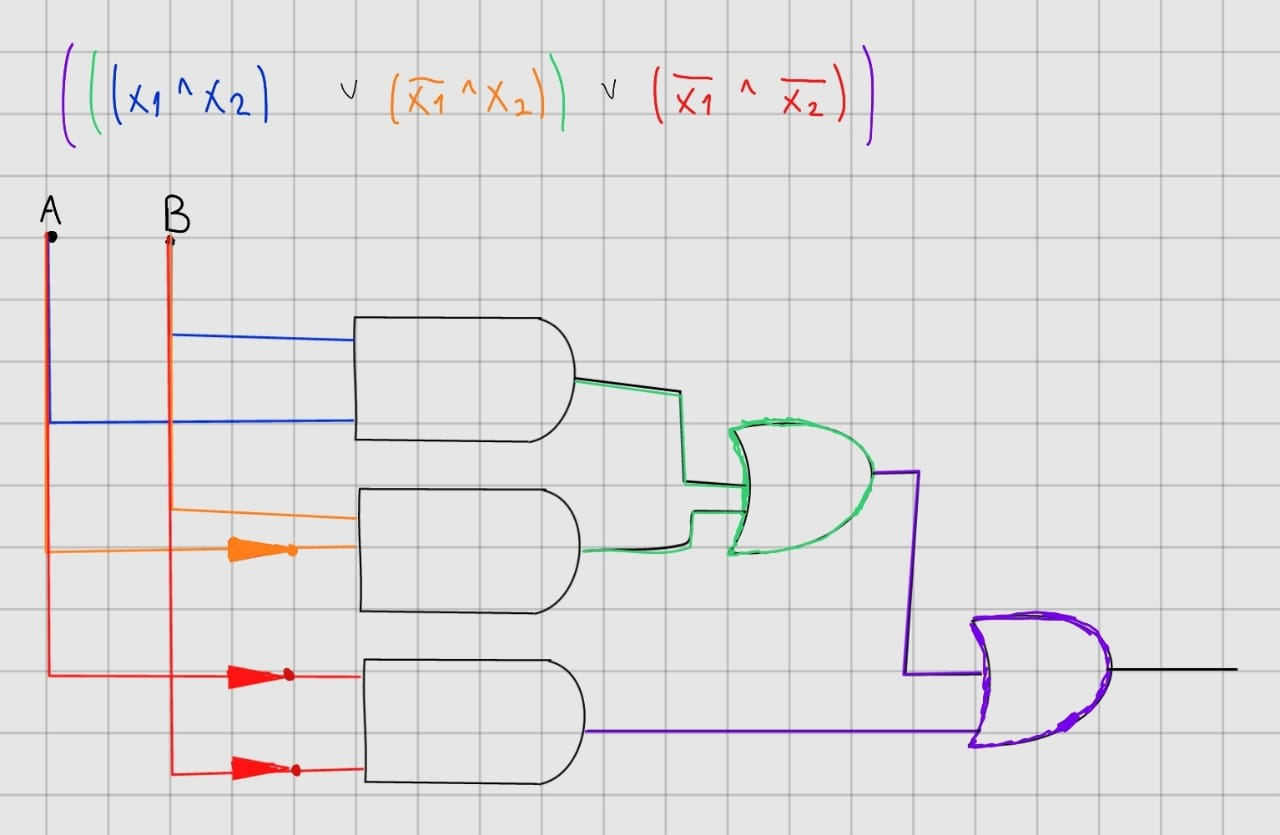
\includegraphics[width=\linewidth]{assets/circuito1.jpg}
    \label{fig:circuito1}
\end{minipage}\]

\subsection*{Carry en circuitos}
El carry debe colocarse en los circuitos en la suma porque en caso de no hacerlo, se nos pierden casos.
\[\begin{minipage}[b]{0.6\textwidth}
    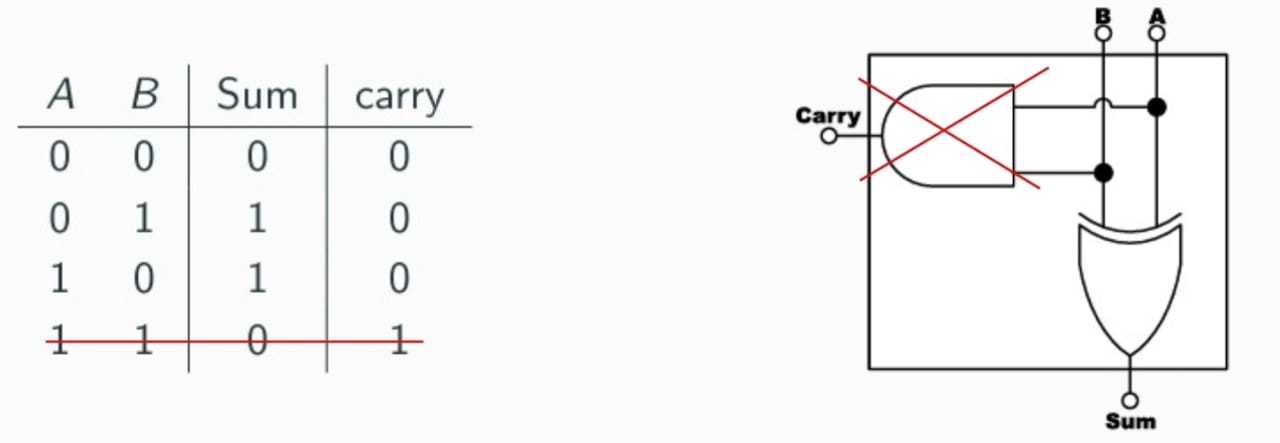
\includegraphics[width=\linewidth]{assets/sin_carry.jpg}
    \label{fig:sin_carry}
\end{minipage}\]

Si eliminamos el carry se nos pierde el caso 1 \( + \) 1, por lo tanto lo ideal sería que al hacer una suma nos quede así: 
\[\begin{minipage}[b]{0.6\textwidth}
    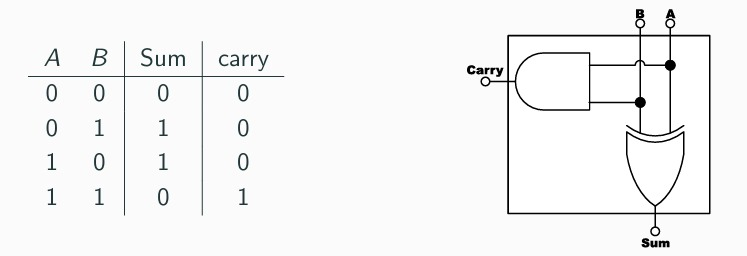
\includegraphics[width=\linewidth]{assets/suma_carry.jpg}
    \label{fig:suma_carry}
\end{minipage}\]

Nota: El carry es representado con un AND porque en la tabla de verdad solo da uno cuando A = 1 y B = 1. Luego, la función Sum es un XOR.

\subsection*{Sumadores}
Los sumadores nos sirven para poder realizar operaciones entre bits.
Es importante recalcar que llamamos half-adder a un sumador de 1 bit, donde solamente tiene una entrada A de 1 bit y una entrada B de 1 bit.
Un sumador de 1 bit requiere:
\begin{itemize}
    \item Dos entradas A y B de 1 bit
    \item Una compuerta XOR (para la suma): solo el resultado es 1 o 0
    \item Una compuerta AND (para el carry): si la suma del XOR es 1+1
\end{itemize} 
\[\begin{minipage}[b]{0.6\textwidth}
    \includegraphics[width=\linewidth]{assets/sumador_1_bit.png}
    \label{fig:sumador_1_bit}
\end{minipage}\]

Veamos un ejemplo con un sumador completo de 3 entradas: Si para dos entradas necesitabamos un sumador simple, para 3 entradas necesito 2. Porque es (A+B) y luego res+C
\[\begin{minipage}[b]{1\textwidth}
    \includegraphics[width=\linewidth]{assets/sumador_completo.png}
    \label{fig:sumador_completo}
\end{minipage}\]
Nótese que para considerar si es carry al final de toda la suma o no usamos un or porque nos basta con que uno haya arrojado carry.

\subsection*{Inversor}
\begin{itemize}
    \item Si me mandan INV=1 entonces tengo que invertir los bits.
    \item La manera de hacer esto es utilizando un XOR.
\end{itemize} 
\[\begin{minipage}[b]{0.6\textwidth}
    \includegraphics[width=\linewidth]{assets/inversor_4_bits.png}
    \label{fig:inversor_4_bits}
\end{minipage}\]


\subsection*{Multiplexor}
Está conformado por varias entradas de control y entradas de datos. Existe una única salida.
\begin{itemize}
    \item Entradas de control: se indican de la manera \(c_{n}\)
    \item Entradas de datos: se indican de la manera \(e_{n}\)
\end{itemize} 
Te ayuda a ahorrar recursos, pero todas las acciones tardan mucho más tiempo porque solo se ejecuta una a la vez. \\
Nos garantiza que la información solo se envía por un único canal. \\
\\
Para poder calcular la cantidad de entradas de control \(c_{n}\) que necesito para una cantidad m de entradas de datos \(e_{m}\) hago el siguiente cálculo: m \(<\) \(2^{l}\) hasta que me pase por primera vez.
\begin{itemize}
    \item Entradas de datos: 30.
    \item Entradas de control: Necesito 5 entradas de control porque \(2^{5}\) es 32.
\end{itemize} 
Cada entrada de control tiene un índice que podemos decirle individuo, por ejemplo, si tengo \(2^{l}\) entradas tengo 32 posibles combinaciones.
\begin{itemize}
    \item Si tengo 00010 significa que la persona que está hablando la persona 2.
\end{itemize}

En los Multiplexores existen difurcaciones, que cuando llegamos a una de ellas se nos desvía el camino enviándonos a una compuerta. Si en algún momento se llega a un valor 0, entonces decimos que el camino ya finalizó.\\
\\
TODO: Añadir imagen

\subsection*{Timing}
En un circuito combinatorio el tiempo que tarda la salida en estabilizarse depende de la cantidad de capas de compuertas (latencia). Para enfrentar el problema usamos secuenciales.

\section*{Latchs}
Utilizan realimentación, es decir, la salida de una compuerta como entrada de otra.
\subsection*{Latch RS}
Tiene dos entradas: S (Set) y R (Reset), y dos salidas, Q y \(\bar{Q}\) y consiste en dos puertas NOR conectadas por realimentación
El circuito es consistente permanece estable \(\iff\) S = R = 0.
Tabla de verdad del Latch
\begin{figure}[h]
    \begin{subfigure}{0.4\textwidth}
        \centering
        \includegraphics[width=0.7\linewidth]{assets/latch_circuito.png}
        \label{fig:latch_circuito}
        \end{subfigure}
    \begin{subfigure}{0.5\textwidth}
        \centering
    \includegraphics[width=0.5\linewidth]{assets/latch.png}
    \label{fig:latch}
    \end{subfigure}
    \end{figure}
    

Funciona como un memorizador
\begin{itemize}
    \item Cuando S está prendido entonces Q = 1.
    \item Cuando Q está prendido entonces \(\bar{Q}\) = 1.
    \item Si ninguno está prendido recuerda el estado anterior. 
    \item Si ambos están prendidos, Q = 0 y \(\bar{Q}\) = 0. Este caso no debería estar permitido porque la salida es inconsistente.
\end{itemize}

Para recordar el estado anterior usamos la notación de: \(Q \ast\) y \(\bar{Q} \ast \) \\

\textbf{Importante}: El valor de las salidas depende de la implementación del latch. Por lo tanto, un Latch con NAND no sería lo mismo que un Latch con NOR.

\subsection*{Latch JK}
Acepta todas las combinaciones posibles de las entradas.
\begin{itemize}
    \item Cuando J está prendido entonces Q = 1.
    \item Cuando K está prendido entonces \(\bar{Q}\) = 1.
    \item Si ninguno está prendido recuerda el estado anterior. 
    \item Si ambos están prendidos, niega el estado anterior (¡necesita que haya un estado anterior!)
\end{itemize}

\[\begin{minipage}[b]{0.8\textwidth}
    \includegraphics[width=\linewidth]{assets/latch_jk.png}
    \label{fig:latch_jk}
\end{minipage}\]

Cuando J y K son 1, la función realizada se denomina función de conmutación, la salida se invierte. 

El circuito oscila (estado inestable)

\subsection*{Latch D}
Es un almacén para un bit de datos. La salida del Latch D es siempre igual al valor más reciente aplicado a la entrada y por lo tanto la recuerda y la produce.

Tiene una entrada de datos y una de control.

Este circuito es estable en todos los estados pero los tiempos no se pueden predecir porque dependen de D y puede causar carreras si existe un lazo en el circuito externo

\begin{itemize}
    \item Cuando D está apagado y C está prendido, se memoriza C.
    \item Si ambos están prendidos, se memoriza D.
    \item En cualquier otro caso, devuelve el valor memorizado.
\end{itemize}

\[\begin{minipage}[b]{0.8\textwidth}
    \includegraphics[width=\linewidth]{assets/latch_d.png}
    \label{fig:latch_d}
\end{minipage}\]

\subsection*{Control de transición de estados: Clock}
\[\begin{minipage}[b]{0.8\textwidth}
    \includegraphics[width=\linewidth]{assets/clock_1.png}
    \label{fig:clock_1}
\end{minipage}\]
El clock que necesitamos utilizar es el 3ro. ¿Por qué? Porque nos interesa solamente memorizar o guardar los estados de los valores cuando el clock está en el pico. \\
No necesitamos estar constantemente escuchando cambios con el clock, sino que nos interesa solo en la subida.
\\
Para solucionar este problema, podemos utilizar un detector de pulso.
\begin{figure}[h]
    \begin{subfigure}{0.4\textwidth}
        \centering
        \includegraphics[width=0.8\linewidth]{assets/detector_pulso_1.png}
        \label{fig:detector_pulso_1}
        \end{subfigure}
    \begin{subfigure}{0.7\textwidth}
        \centering
    \includegraphics[width=0.6\linewidth]{assets/detector_pulso_2.png}
    \caption{Detector de pulso implementado usando una compuerta AND. }
    \label{fig:detector_pulso_2}
    \end{subfigure}
    \end{figure}
\\ Es importante notar, que el detector de pulso dará 1 (el pico) en algunos casos porque la compuerta NOT tiene un pequeño delay para poder negar la entrada. A continuación se muestra un ejemplo de esto.
\[\begin{minipage}[b]{0.6\textwidth}
    \includegraphics[width=\linewidth]{assets/detector_pulso_3.png}
    \label{fig:detector_pulso_3}
\end{minipage}\]
La línea punteada indica el tiempo que tardó la entrada en ser negada. En ese momento es donde se nos ejecutan los picos que nosotros necesitamos. \\
Si mandamos input = 1, el primer momento queda 1 AND 1 y el AND es verdadero, pero luego de un momento queda 1 AND 0 y ahora la señal vuelve a estar baja. Si fuese 1 AND 1 todo el tiempo tendríamos un clock constante y no necesitamos eso. \\
Todas las compuertas tienen delay porque al estar compuestas de silicio, tardan un poco en entrar en calor.

\subsection*{Flip-Flop JK}
Está armado en base a Latch JK + Clock. \\
El Latch JK funcionará igual pero solo memorizará el valor sii el clock está en el flanco de subida.
\begin{itemize}
    \item Cuando J es 1 y el clock está prendido, se guarda el valor de J.
    \item Cuando K es 1 y el clock está prendido, se guarda el valor de K.
    \item Cuando el clock está apagado devuelve el valor de J/K guardado en el último pulso al clock. 
    \item Cuando el clock está apagado y J, K = 1 se niega el resultado guardado en el último pulso al clock.
    \item En cualquier otro caso, sucede el ítem anterior.
\end{itemize}
\subsection*{Flip-Flop D}
Está armado en base a Latch D + Clock. \\
El Latch D funcionará igual pero solo memorizará el valor sii el clock está en el flanco de subida.
\begin{itemize}
    \item Cuando el clock es 1, guarda el valor de D en ese instante.
    \item Cuando el clock está apagado, devuelve el valor de D guardado en el último pulso al clock. En criollo: Guarda el valor de D hasta que haya otro flanco de subida (ciclo) y guarde uno nuevo.
\end{itemize}

\[\begin{minipage}[b]{0.8\textwidth}
    \includegraphics[width=\linewidth]{assets/flip_flop_d.png}
    \label{fig:flip_flop_d}
\end{minipage}\]

Nota: \(1\uparrow\) indica que solo es se evalúa cuando está en el flanco de subida.
\subsection*{Registros}
Para poder escribir registros necesitamos una entrada de control Enable que nos permitirá decirle al Flip-Flop cuando nosotros queremos permitir que nos cambie el valor / escriba la memoria. \\
Este flag de Enable deberá ir en un AND con el Clock, entonces si Enable = 1 y el Clock está en 1, entonces se le permite al Flip Flop guardar el valor de la operación realizada.
\[\begin{minipage}[b]{0.6\textwidth}
    \includegraphics[width=\linewidth]{assets/flip_flop_d_enable.png}
    \label{fig:flip_flop_d_enable}
\end{minipage}\]

Recuerdo: El Flip Flop D solo almacena 1 bit. Si necesitaramos almacenar n bits (registro de n bits) necesitaríamos n Flip Flop D y UN solo Enable/Clock.



\end{document}